\documentclass[10pt,a5paper,openany]{book}

\usepackage{palatino}
\usepackage[outer=1.0cm,inner=1.8cm,top=1.5cm,bottom=1.3cm]{geometry}
\usepackage[portuguese]{babel}
\usepackage[colorlinks=true,linkcolor=black]{hyperref}
\usepackage{graphicx}

\usepackage{fancyhdr}
\fancyhf{}
\fancyhead[LE,RO]{\thepage}
\fancyhead[RE,LO]{\small SONGBOOK -- Legião Urbana}
\fancyfoot[C]{\footnotesize \copyright ~ \the\year ~ Samuel Santana da Purificação}
\fancyfoot[LE,RO]{\thepage}
\renewcommand{\headrulewidth}{1pt}
\renewcommand{\footrulewidth}{1pt}
\pagestyle{fancy}

\usepackage[onesongcolumn]{songs}
\renewcommand{\idxtitlefont}{\normalsize}
\renewcommand{\idxrefsfont}{\normalsize}
\setlength{\songnumwidth}{1cm}
\renewcommand{\printsongnum}[1]{\bfseries\huge #1}
\renewcommand{\stitlefont}{\bfseries\LARGE}
\renewcommand{\extendprelude}{\small\showrefs\showauthors{\itshape\songcopyright\par}}
\renewcommand{\printchord}[1]{\bfseries\normalsize#1}
\renewcommand{\clineparams}{\baselineskip=10pt}
\renewcommand{\sharpsymbol}{\#}
\renewcommand{\flatsymbol}{b}
\setlength{\cbarwidth}{1pt}
\setlength{\sbarheight}{0pt}
\renewcommand{\makepostlude}{\resettitles}
\minfrets=5

\title{\bfseries\Huge SONGBOOK\\LEGIÃO URBANA\\
\vfill
\begin{figure}[h]
		\centering
		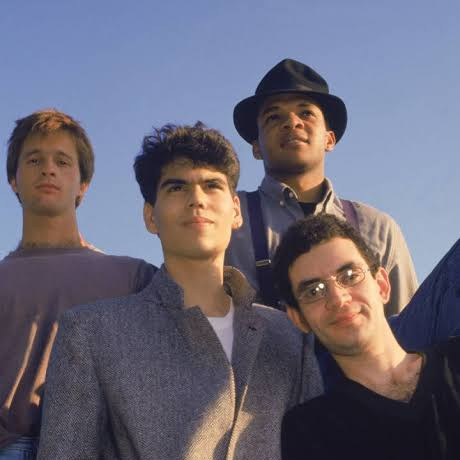
\includegraphics[width=0.4\textwidth]{img.jpg}
\end{figure}
\vfill}
\author{Samuel Santana da Purificação}
\date{\small\today}

\newindex{index}{index}
\indexsongsas{index}{\thepage}

\begin{document}

\newgeometry{margin=1.5cm}
\maketitle
\thispagestyle{empty}
\restoregeometry
\null
\showindex[2]{\rmfamily Índice}{index}

\begin{songs}{index}
	\beginsong{Será}[
	by={Dado Villa-Lobos, Marcelo Bonfá, Renato Russo e Renato Rocha},
	cr={\copyright~Legião Urbana - Álbum: Legião Urbana (1985)}]

\beginverse*
\nolyrics Introdução: \[C] \[G] \[Am] \[F] \rep{2}
\endverse

\beginverse
\[C] Tire suas \[G]mãos de mim \[Am] eu não per\[F]tenço a você
\[C] Não é me domi\[G]nando assim \[Am] que você \[F]vai me entender
\[C] Eu posso estar so\[G]zinho \[Am] mas, eu sei muito \[F]bem aonde estou
\[Am] Você pode até \[G]duvidar \[F] acho que isso não \[G]é amor
\endverse

\beginverse*
\nolyrics Arranjo: \[C] \[F] \[G] \rep{4}
\endverse

\beginchorus
\[G]Será só imagina\[Dm]ção
\[G]Será que nada vai a\[Dm]contecer
\[G]Será que é tudo isso em \[Dm]vão
\[G]Será que vamos conse\[Dm]guir venc\[Am]er ô\[F]ôôôô\[G]ô
\endchorus

\beginverse*
\nolyrics Arranjo: \[C] \[F] \[G] \rep{4}
\endverse

\beginverse
\[C] Nos perderemos entre \[G]monstros \[Am] da nossa própria \[F]criação
\[C] Serão noites in\[G]teiras \[Am] talvez por medo da es\[F]curidão
\[C] Ficaremos acor\[G]dados \[Am] imaginando alguma \[F]solução
\[Am] Pra que esse nosso ego\[G]ísmo \[F] não destrua nosso \[G]coração
\endverse

\beginverse*
\nolyrics Arranjo: \[C] \[F] \[G] \rep{4}
\endverse

\beginchorus
\[G]Será só imagina\[Dm]ção
\[G]Será que nada vai a\[Dm]contecer
\[G]Será que é tudo isso em \[Dm]vão
\[G]Será que vamos conse\[Dm]guir venc\[Am]er ô\[F]ôôôô\[G]ô
\endchorus

\beginverse
Bri\[C]gar pra quê, se é \[G/B]sem querer
Quem \[B&]é que vai nos \[Dm]proteger
Se\[C]rá que vamos ter que \[G/B]responder
Pelos \[B&]erros a mais \[Dm]Eu e você
\endverse

\beginverse*
\nolyrics Final: \[G] \[F] \rep{4} ~ \[F]
\endverse

\vspace{20pt}
\gtab{C}{X32010:032010}
\gtab{Dm}{XX0231:000231}
\gtab{F\vspace{5pt}}{(133211):134211}
\gtab{G}{320033:210034}
\gtab{G/B}{X20033:010034}
\gtab{Am}{X02210:002310}
\gtab{B&}{X(13331):012341}

\endsong

	\beginsong{Tempo Perdido}[
	by={Renato Russo},
	cr={\copyright~Legião Urbana - Álbum: Dois (1986)}]

\beginverse*
\nolyrics Introdução: \[C] \[Am7] \[Bm7] \[Em7]
\endverse

\beginverse
Todos os \[C]dias quando acordo \[Am7]
\[Bm7] Não tenho mais o \[Em7]tempo que passou
Mas tenho \[C]muito tempo \[Am7]
Temos \[Bm7]todo o tempo do \[Em7]mundo
\[C] Todos os dias \[Am7]antes de dormir
\[Bm7]Lembro e esqueço como foi o \[Em7]dia
\endverse

\beginverse
\[C]Sempre em frente\[Am7]
Não \[Bm]temos tempo a per\[Em7]der
Nosso su\[C]or sagrado\[Am7]
É bem mais \[Bm7]belo que esse sangue a\[Em7]margo
E tão \[C]sério - \[Am7]o
\endverse

\beginverse*
E sel\[Bm7]va\[Em7]gem \rep{3}
\endverse

\beginverse*
\nolyrics Solo: \[Em7] \[Bm7] \rep{4} \[~Em7]
\endverse

\beginverse
\[C]Veja o sol dessa ma\[Am7]nhã tão cinza \[Bm7]
A tempes\[Em7]tade que chega é da \[C]cor dos teus olhos\[Am7]
Cas\[Bm7]ta\[Em7]nhos
Então me a\[C]braça forte\[Am7] e \[Bm7]diz mais uma vez
Que já es\[Em7]tamos dis\[C]tantes de \[Am7]tudo
\endverse

\beginverse*
\[Bm7]Temos nosso próprio \[Em7]tempo \rep{3}
\endverse

\beginverse
Não \[C]tenho medo \[Am7] do escuro
\[Bm7] Mas deixe \[Em7]   as luzes \[C]  acesas \[Am7]
Ag\[Bm7]o\[Em7]ra!
O que \[C]foi escondido é o \[Am7]que se escondeu
E o que \[Bm7]foi prometido nin\[Em7]guém prometeu
Nem foi \[C]tempo perdido\[Am7]
\endverse

\beginverse*
Somos tão \[Bm7]jo\[Em7]vens \rep{3}
\endverse

\beginverse*
\nolyrics Final: \[C] \[Am7] \[Bm7] \[Em7] \rep{4}
\endverse

\vspace{20pt}
\gtab{C}{X32010:032010}
\gtab{Em7}{022030:012030}
\gtab{Am7}{X02010:002010}
\gtab{Bm7}{X(24232):014121}

\endsong

	\beginsong{Pais e Filhos}[
    by={Dado Villa-Lobos, Marcelo Bonfá e Renato Russo},
    cr={\copyright~Legião Urbana - Álbum: As Quatro Estações (1989)}]

\beginverse*
\nolyrics Introdução: \[C] \[D] \[G] \rep{4}
\endverse

\beginverse
Es\[C]tátuas e \[D] cofres e pa\[G]redes pintadas ninguém \[C]sabe o que \[D]aconte\[G]ceu
\[C]Ela se \[D]jogou da ja\[G]nela do quinto andar \[C]nada é fácil \[D]de enten\[G]der \[C D]
\endverse

\beginverse*
\[Fadd9]   Dorme a\[Em]gora \[C]
\[Bm7]Uhmhum! \[Am7] é só o vento lá \[D]fora
\endverse

\beginverse
\[C] Quero \[D] colo, \[G]Vou fugir de casa, p\[C]osso dor\[D]mir aqui \[G]com vocês
\[C] Estou \[D]com medo \[G]tive um pesadelo, \[C] só vou \[D]Voltar depois \[G] das três \[C D]
\endverse

\beginverse*
\[Fadd9]  Meu \[Em]filho vai ter \[C]
Nome de \[Bm7]santo \[Am7]Uhmhum! quero o nome mais \[D] bonito
\endverse

\beginchorus
É pre\[G]ciso ama - \[C]ar as pessoas
Como \[Em]se não houvesse ama\[C]nhã
Porque se \[G]você para - \[C]ar pra pensar
\[Em] Na verdade não \[C]há
\endchorus

\beginverse
\[C] Me diz\[D], \[G] por que que o céu\[C] é  a\[D]zul
\[G] Explica a grande \[C]fúria \[D]do mundo \[G] \[C D G]
São meus \[C]filhos que \[D] tomam \[G]conta de mim \[C D G]
Eu moro com a \[C]minha mãe\[D] mas meu pai \[G]vem me visitar \[C D G]
Eu moro na \[C] rua não \[D] tenho nin\[G]guém
Eu \[C]moro em qualquer \[D] lugar \[G]
Já mo\[C]rei em tanta \[D] casa que nem \[G] me lembro mais
\endverse

\beginverse*
\[C] Eu moro \[D] com os meus \[Fadd9]pais \[Em] \[C] \[Bm7]Uhmhum! \[Am7] \[D]ouh!\\
\endverse

\beginchorus
É pre\[G]ciso ama - \[C]ar as pessoas Como \[Em]se não houvesse ama\[C]nhã
Porque se \[G]você para - \[C]ar pra pensar \[Em] Na verdade não \[C]há
\[G]Sou uma gota d'água\[C] \[Em]Sou um grão de areia - \[C]a
Você me \[G]diz que seus pais não en\[C]tendem
Mas vo\[Em]cê não entende seus \[C] pais
\endchorus

\beginverse
Você \[C]culpa seus \[D] pais por \[G]tudo, \[C]Isso é a\[D]bsurdo \[G]
São cri\[C]anças \[D] como vo\[G]cê.
O que vo\[C]cê vai \[G]ser quando vo\[G]cê crescer?
\endverse

\beginverse*
\nolyrics Final: \[C] \[D] \[G] \rep{4}
\endverse

\vspace{20pt}
\gtab{C}{X32010:032010}
\gtab{D}{XX0232:000132}
\gtab{Em}{022000:012000}
\gtab{Fadd9}{XX3213:003214}
\gtab{G}{320033:320034}
\gtab{Am7}{X02010:002010}
\gtab{Bm7}{X(24232):014121}

\endsong
	\beginsong{Vento No Litoral}[
	by={Renato Russo},
	cr={\copyright~Legião Urbana - Álbum: V (1991)}]

\beginverse*
\nolyrics Introdução: \[Am] \[Em] \[Am] \[Em] \[F] \[C] \[F] \[C]
\endverse

\beginverse
De \[Am]tarde quero descansar, che\[Em]gar até a praia e ver
Se o \[Am]vento ainda está forte, e vai ser \[Em]bom subir nas pedras
Sei que \[C]faço isso pra esquecer, eu \[B&sus2]deixo a onda me acertar
E o \[Am]vento vai levando tudo em\[F]bor\[G]a
\endverse

\beginverse*
\nolyrics Arranjo: \[Am] \[F] \[G] \[C]
\endverse

\beginverse
\[F] Agora está tão \[Em]longe ver a linha do hori\[Dm]zonte me distrai
Dos nossos \[(G]planos \[Am] é que \[G/B)]tenho mais sau\[F]dade
Quando olhávamos \[Em]juntos na mesma direção \[Dm]
Aonde es\[B&sus2]tá você agora além de a\[Am]qui dentro de \[F]mim?\[G]
\endverse

\beginverse*
\nolyrics Arranjo: \[F] \[G] \[Am] \rep{2}
\nolyrics Solo: \[Am] \[Em] \[Am] \[Em] \[C] \[B&sus2] \[Am] \[F] \[G Am] \[F] \[G]
\endverse

\beginverse*
\[Cm] Agimos certo sem querer
\[G/B] Foi só o tempo que errou
\[Gm7/B&] Vai ser difícil sem você
Porq\[A7sus4]ue você está co\[A7]migo o tempo \[Dm]todo quando vejo o mar
\[C] Existe algo que diz:
A \[G/B]vida conti\[Am]nua e se entre\[G]gar é uma bo\[F]bagem
\endverse

\beginchorus
\[Em]Já que vo\[A7]cê não está aqui \[Dm]
O que posso fazer \[Dm/C] é cui\[B&sus2]dar de mim\[G]
Quero \[C]ser feliz ao menos \[F]
Lembra que o \[B&sus2]plano era fi\[G]carmos bem?
\endchorus

\beginverse*
\[Am]Eieieieiei \[Em]  olha só o que eu a\[Am]chei \[(G Am G/B G/D)]
\[C]  Cavalos-marinhos\[F]\[Esus4]\[E]
\endverse

\beginverse*
\nolyrics Solo: \[Am] \[Em] \[Am] \[Em]
\endverse

\beginverse
Sei que \[C]faço isso pra esquecer, eu \[B&sus2]deixo a onda me acertar
E o \[Am]vento vai levando tudo em\[F]bor\[G]a
\endverse

\beginverse*
\nolyrics Final: \[C] \[F] \rep{4}
\endverse

\vspace{20pt}
\gtab{C}{X32010:032010}
\gtab{Cm}{X(35543):014321}
\gtab{Dm}{XX0231:000231}
\gtab{Dm/C}{X3X231:040231}
\gtab{E}{022100:023100}
\gtab{Esus4}{022200:023400}
\gtab{Em}{022000:012000}
\gtab{F\vspace{5pt}}{(133211):134211}\\
\gtab{G}{320033:210034}
\gtab{G/D}{XX0033:000034}
\gtab{G/B}{X20033:010034}
\gtab{Gm7/B&}{X1X333:010234}
\gtab{A7}{X02020:002030}
\gtab{A7sus4}{X02030:002040}
\gtab{Am}{X02210:002310}
\gtab{B&sus2}{X(13311):013411}

\endsong

	\beginsong{Mais Uma Vez}[
    by={Renato Russo, Flávio Venturini},
    cr={\copyright~Legião Urbana - Single: Mais Uma Vez (2003)}]

\capo{1}

\beginverse*
\nolyrics Introdução: \[Asus2] \rep{4}
\endverse

\beginchorus
Mas é \[Asus2]claro que o sol vai vol\[B(11)]tar amanhã
Mais uma \[C#m7]vez, eu \[(F#m7(11)]sei \[B7sus4]\[Esus4]\[E)]
Escuri\[Asus2]dão já vi pior de endoide\[B(11)]cer gente sã
Espera que o \[C#m7]sol já \[(F#m7(11)]vem \[B7sus4]\[Esus4]\[E)]
\endchorus

\beginverse
\[Asus2] Tem gente que está do mesmo lado
que vo\[Asus2]cê mas deveria estar do lado de lá
\[F#m7(11)] Tem gente que machuca os outros
\[D6sus2] Tem gente que não \[Bm7(11)]sabe a\[E]mar
\[Asus2] Tem gente enganando a gente \[F#m7(11)]{ ~~ veja nossa vida como está}
\[D6sus2] Mas eu sei que um dia a \[Bm7(11)]gente a\[E]prende
\[Asus2] Se você quiser alguém em quem confi\[F#m7(11)]ar
Confie em si mesmo \[D6sus2] Quem acredita \[Bm7(11)]sempre al\[E]cança
\endverse

\beginverse*
\nolyrics Solo: \[Asus2] \rep{3}
\endverse

\beginchorus
Mas é \[Asus2]claro que o sol vai vol\[B(11)]tar amanhã
Mais uma \[C#m7]vez, eu \[(F#m7(11)]sei \[B7sus4]\[Esus4]\[E)]
Escuri\[Asus2]dão já vi pior \[Aaug] de endoide\[B(11)]cer gente sã
Espera que o \[C#m7]sol já \[(F#m7(11)]vem \[B7sus4]\[Esus4]\[E)]
\endchorus

\beginverse
\[Asus2] Nunca deixe que lhe digam que não vale a
\[Asus2]pena acreditar no sonho que se tem
\[F#m7(11)] Ou que seus planos nunca vão dar certo
\[D6sus2] Ou que você nunca vai \[Bm7(11)]ser al\[E]guém
\[Asus2] Tem gente que machuca os outros
\[F#m7(11)] Tem gente que não sabe amar
\[D6sus2] Mais um dia a \[Bm7(11)]gente a\[E]prende
\[Asus2] Se você quiser alguém em quem confi\[F#m7(11)]ar
Confie em si mesmo \[D6sus2] Quem acredita \[Bm7(11)]sempre al\[E]cança
\endverse

\beginverse*
\nolyrics Solo: \[Asus2] \[F#m7(11)] \[D6sus2] \[Bm7(11)] \[E]
\endverse

\beginverse*
\[Asus2] Quem acredita sempre alcança
\[F#m7(11)] Quem acredita sempre alcança
\[D6sus2] Quem acredita \[Bm7(11)]sempre al\[E]cança
\endverse

\beginverse*
\nolyrics Final: \[Asus2] \rep{5}
\endverse

\vspace{20pt}
\gtab{C#m7}{4:X(13121):013121}
\gtab{D6sus2}{XX0200:000200}
\gtab{E}{022100:023100}
\gtab{Esus4}{022200:012300}
\gtab{F#m7(11)}{2X220X:203400}
\gtab{Asus2}{X02200:002300}
\gtab{Aaug}{X03221:004231}
\gtab{B(11)}{X24440:012340}\\
\gtab{B7sus4}{X22200:012300}
\gtab{Bm7(11)}{X20230:010230}

\endsong
	\beginsong{Que País É Este?}[
	by={Renato Russo},
	cr={\copyright~Legião Urbana - Álbum: Que País É Este 1978/1987 (1987)}]

\beginverse*
\nolyrics Introdução: \[Em] \[C] \[D] \rep{12}
\endverse

\beginverse
Nas fa\[Em]velas, no se\[C]nado \[D]
\[Em]   Sujeira pra todo \[C]lado \[D]
Ninguém res\[Em]peita a constitui\[C]ção \[D]
Mas \[Em]todos acreditam no fu\[C]turo da na\[D]ção \[~ (Em] \[C] \[D)]\\
\endverse

\beginchorus
Que pa\[Em]ís é esse \[C] \[D]
Que pa\[Em]ís é esse \[C] \[D]
Que pa\[Em]ís é esse \[C] \[D]
\endchorus

\beginverse*
\nolyrics Solo: \[Em] \[C] \[D] \rep{4}
\endverse

\beginverse
No Ama\[Em]zonas, no Ara\[C]guaia iá iá i\[D]á
Na bai\[Em]xada fluminense \[C] \[D]
Mato \[Em]Grosso, Minas Ge\[C]rais \[D]
E no nor\[Em]deste tudo em paz \[C] \[D]
Na morte \[Em]eu descanso \[C] \[D]
Mas o \[Em]sangue anda solto \[C] \[D]
Manchando \[Em]os papéis \[C] \[D]
Docu\[Em]mentos fiéis \[C] \[D]
Ao des\[Em]canso do patrão \[C] \[D]
\endverse

\beginchorus
Que pa\[Em]ís é esse \[C] \[D]
Que pa\[Em]ís é esse \[C] \[D]
Que pa\[Em]ís é esse \[C] \[D]
\endchorus

\beginverse*
\nolyrics Solo: \[Em] \[C] \[D] \rep{4}
\endverse

\beginverse
Terceiro \[Em]mundo se for \[C] \[D]
Piada \[Em]no exterior \[C] \[D]
Mas o Bra\[Em]sil vai ficar rico \[C] \[D]
Vamos fatu\[Em]rar um milhão \[C] \[D]
Quando ven\[Em]dermos todas as \[C]almas \[D]
Dos nossos \[Em]índios num leilão \[C] \[D]
\endverse

\beginchorus
Que pa\[Em]ís é esse \[C] \[D]
Que pa\[Em]ís é esse \[C] \[D]
Que pa\[Em]ís é esse \[C] \[D]
\endchorus

\vspace{20pt}
\gtab{C}{X32010:032010}
\gtab{D}{XX0232:000132}
\gtab{Em}{022000:012000}


\endsong

\end{songs}

\end{document}
